% Options for packages loaded elsewhere
\PassOptionsToPackage{unicode}{hyperref}
\PassOptionsToPackage{hyphens}{url}
\PassOptionsToPackage{dvipsnames,svgnames,x11names}{xcolor}
%
\documentclass[
  letterpaper,
  DIV=11,
  numbers=noendperiod]{scrreprt}

\usepackage{amsmath,amssymb}
\usepackage{iftex}
\ifPDFTeX
  \usepackage[T1]{fontenc}
  \usepackage[utf8]{inputenc}
  \usepackage{textcomp} % provide euro and other symbols
\else % if luatex or xetex
  \usepackage{unicode-math}
  \defaultfontfeatures{Scale=MatchLowercase}
  \defaultfontfeatures[\rmfamily]{Ligatures=TeX,Scale=1}
\fi
\usepackage{lmodern}
\ifPDFTeX\else  
    % xetex/luatex font selection
\fi
% Use upquote if available, for straight quotes in verbatim environments
\IfFileExists{upquote.sty}{\usepackage{upquote}}{}
\IfFileExists{microtype.sty}{% use microtype if available
  \usepackage[]{microtype}
  \UseMicrotypeSet[protrusion]{basicmath} % disable protrusion for tt fonts
}{}
\makeatletter
\@ifundefined{KOMAClassName}{% if non-KOMA class
  \IfFileExists{parskip.sty}{%
    \usepackage{parskip}
  }{% else
    \setlength{\parindent}{0pt}
    \setlength{\parskip}{6pt plus 2pt minus 1pt}}
}{% if KOMA class
  \KOMAoptions{parskip=half}}
\makeatother
\usepackage{xcolor}
\setlength{\emergencystretch}{3em} % prevent overfull lines
\setcounter{secnumdepth}{5}
% Make \paragraph and \subparagraph free-standing
\ifx\paragraph\undefined\else
  \let\oldparagraph\paragraph
  \renewcommand{\paragraph}[1]{\oldparagraph{#1}\mbox{}}
\fi
\ifx\subparagraph\undefined\else
  \let\oldsubparagraph\subparagraph
  \renewcommand{\subparagraph}[1]{\oldsubparagraph{#1}\mbox{}}
\fi


\providecommand{\tightlist}{%
  \setlength{\itemsep}{0pt}\setlength{\parskip}{0pt}}\usepackage{longtable,booktabs,array}
\usepackage{calc} % for calculating minipage widths
% Correct order of tables after \paragraph or \subparagraph
\usepackage{etoolbox}
\makeatletter
\patchcmd\longtable{\par}{\if@noskipsec\mbox{}\fi\par}{}{}
\makeatother
% Allow footnotes in longtable head/foot
\IfFileExists{footnotehyper.sty}{\usepackage{footnotehyper}}{\usepackage{footnote}}
\makesavenoteenv{longtable}
\usepackage{graphicx}
\makeatletter
\def\maxwidth{\ifdim\Gin@nat@width>\linewidth\linewidth\else\Gin@nat@width\fi}
\def\maxheight{\ifdim\Gin@nat@height>\textheight\textheight\else\Gin@nat@height\fi}
\makeatother
% Scale images if necessary, so that they will not overflow the page
% margins by default, and it is still possible to overwrite the defaults
% using explicit options in \includegraphics[width, height, ...]{}
\setkeys{Gin}{width=\maxwidth,height=\maxheight,keepaspectratio}
% Set default figure placement to htbp
\makeatletter
\def\fps@figure{htbp}
\makeatother
\newlength{\cslhangindent}
\setlength{\cslhangindent}{1.5em}
\newlength{\csllabelwidth}
\setlength{\csllabelwidth}{3em}
\newlength{\cslentryspacingunit} % times entry-spacing
\setlength{\cslentryspacingunit}{\parskip}
\newenvironment{CSLReferences}[2] % #1 hanging-ident, #2 entry spacing
 {% don't indent paragraphs
  \setlength{\parindent}{0pt}
  % turn on hanging indent if param 1 is 1
  \ifodd #1
  \let\oldpar\par
  \def\par{\hangindent=\cslhangindent\oldpar}
  \fi
  % set entry spacing
  \setlength{\parskip}{#2\cslentryspacingunit}
 }%
 {}
\usepackage{calc}
\newcommand{\CSLBlock}[1]{#1\hfill\break}
\newcommand{\CSLLeftMargin}[1]{\parbox[t]{\csllabelwidth}{#1}}
\newcommand{\CSLRightInline}[1]{\parbox[t]{\linewidth - \csllabelwidth}{#1}\break}
\newcommand{\CSLIndent}[1]{\hspace{\cslhangindent}#1}

\KOMAoption{captions}{tableheading}
\makeatletter
\@ifpackageloaded{tcolorbox}{}{\usepackage[skins,breakable]{tcolorbox}}
\@ifpackageloaded{fontawesome5}{}{\usepackage{fontawesome5}}
\definecolor{quarto-callout-color}{HTML}{909090}
\definecolor{quarto-callout-note-color}{HTML}{0758E5}
\definecolor{quarto-callout-important-color}{HTML}{CC1914}
\definecolor{quarto-callout-warning-color}{HTML}{EB9113}
\definecolor{quarto-callout-tip-color}{HTML}{00A047}
\definecolor{quarto-callout-caution-color}{HTML}{FC5300}
\definecolor{quarto-callout-color-frame}{HTML}{acacac}
\definecolor{quarto-callout-note-color-frame}{HTML}{4582ec}
\definecolor{quarto-callout-important-color-frame}{HTML}{d9534f}
\definecolor{quarto-callout-warning-color-frame}{HTML}{f0ad4e}
\definecolor{quarto-callout-tip-color-frame}{HTML}{02b875}
\definecolor{quarto-callout-caution-color-frame}{HTML}{fd7e14}
\makeatother
\makeatletter
\makeatother
\makeatletter
\@ifpackageloaded{bookmark}{}{\usepackage{bookmark}}
\makeatother
\makeatletter
\@ifpackageloaded{caption}{}{\usepackage{caption}}
\AtBeginDocument{%
\ifdefined\contentsname
  \renewcommand*\contentsname{Table of contents}
\else
  \newcommand\contentsname{Table of contents}
\fi
\ifdefined\listfigurename
  \renewcommand*\listfigurename{List of Figures}
\else
  \newcommand\listfigurename{List of Figures}
\fi
\ifdefined\listtablename
  \renewcommand*\listtablename{List of Tables}
\else
  \newcommand\listtablename{List of Tables}
\fi
\ifdefined\figurename
  \renewcommand*\figurename{Figure}
\else
  \newcommand\figurename{Figure}
\fi
\ifdefined\tablename
  \renewcommand*\tablename{Table}
\else
  \newcommand\tablename{Table}
\fi
}
\@ifpackageloaded{float}{}{\usepackage{float}}
\floatstyle{ruled}
\@ifundefined{c@chapter}{\newfloat{codelisting}{h}{lop}}{\newfloat{codelisting}{h}{lop}[chapter]}
\floatname{codelisting}{Listing}
\newcommand*\listoflistings{\listof{codelisting}{List of Listings}}
\makeatother
\makeatletter
\@ifpackageloaded{caption}{}{\usepackage{caption}}
\@ifpackageloaded{subcaption}{}{\usepackage{subcaption}}
\makeatother
\makeatletter
\@ifpackageloaded{tcolorbox}{}{\usepackage[skins,breakable]{tcolorbox}}
\makeatother
\makeatletter
\@ifundefined{shadecolor}{\definecolor{shadecolor}{rgb}{.97, .97, .97}}
\makeatother
\makeatletter
\makeatother
\makeatletter
\makeatother
\ifLuaTeX
  \usepackage{selnolig}  % disable illegal ligatures
\fi
\IfFileExists{bookmark.sty}{\usepackage{bookmark}}{\usepackage{hyperref}}
\IfFileExists{xurl.sty}{\usepackage{xurl}}{} % add URL line breaks if available
\urlstyle{same} % disable monospaced font for URLs
\hypersetup{
  pdftitle={The science needed for robust, scalable, and credible nature-based climate solutions in the United States},
  pdfauthor={William Anderegg; Dave Hollinger; Marcy Litvak; Caroline Normile; Gyami Shrestha; Maya Almaraz; Christa Anderson; Mallory Barnes; Dennis Baldocchi; Lily Colburn; Danny Cullenward; Margaret Evans; Kaiyu Guan; Trevor Keenan; Rachel Lamb; Elizabeth Larson; Emily Oldfield; Benjamin Poulter; Julian Reyes; Jonathan Sanderman; Paul Selmants; Edil Sepulveda Carlo; Margaret Torn; Anna Trugman; Christopher Woodall},
  colorlinks=true,
  linkcolor={blue},
  filecolor={Maroon},
  citecolor={Blue},
  urlcolor={Blue},
  pdfcreator={LaTeX via pandoc}}

\title{The science needed for robust, scalable, and credible
nature-based climate solutions in the United States}
\usepackage{etoolbox}
\makeatletter
\providecommand{\subtitle}[1]{% add subtitle to \maketitle
  \apptocmd{\@title}{\par {\large #1 \par}}{}{}
}
\makeatother
\subtitle{Full Report}
\author{Kim Novick \and Christopher Williams \and Benjamin
Runkle \and William Anderegg \and Dave Hollinger \and Marcy
Litvak \and Caroline Normile \and Gyami Shrestha \and Maya
Almaraz \and Christa Anderson \and Mallory Barnes \and Dennis
Baldocchi \and Lily Colburn \and Danny Cullenward \and Margaret
Evans \and Kaiyu Guan \and Trevor Keenan \and Rachel Lamb \and Elizabeth
Larson \and Emily Oldfield \and Benjamin Poulter \and Julian
Reyes \and Jonathan Sanderman \and Paul Selmants \and Edil Sepulveda
Carlo \and Margaret Torn \and Anna Trugman \and Christopher Woodall}
\date{2022-10-12}

\begin{document}
\maketitle
\ifdefined\Shaded\renewenvironment{Shaded}{\begin{tcolorbox}[sharp corners, interior hidden, frame hidden, enhanced, boxrule=0pt, borderline west={3pt}{0pt}{shadecolor}, breakable]}{\end{tcolorbox}}\fi

\renewcommand*\contentsname{Table of contents}
{
\hypersetup{linkcolor=}
\setcounter{tocdepth}{2}
\tableofcontents
}
\bookmarksetup{startatroot}

\hypertarget{front-matter}{%
\chapter*{Front Matter}\label{front-matter}}
\addcontentsline{toc}{chapter}{Front Matter}

\markboth{Front Matter}{Front Matter}

This report emerged from a workshop in Washington, DC, June 28-29th,
2022. Workshop funding and programmatic support came from the Department
of Energy's
\href{https://ameriflux.lbl.gov/about/ameriflux-management-project/}{AmeriFlux
Management Project}, \href{https://oneill.indiana.edu/}{Indiana
University's O'Neill School of Public and Environmental Affairs}, and
the \href{https://www.carboncyclescience.us/}{US Carbon Cycle Science
Program}.

The views expressed in this report do not necessarily reflect the views
of individual contributing authors or their respective institutions.

\hypertarget{acknowledgements}{%
\section*{Acknowledgements}\label{acknowledgements}}
\addcontentsline{toc}{section}{Acknowledgements}

\markright{Acknowledgements}

The report authors are grateful for the support provided by the
\href{https://oneill.indiana.edu/}{Indiana University O'Neill School of
Public and Environmental Affairs}, the AmeriFlux Management Project, and
the U.S. Carbon Cycle Science Program for supporting the workshop and
the writing process. We especially acknowledge Katherine Devich and
Nikki Rolf Boyd for logistical support during the workshop, and Christin
Buechner for programmatic support leading up to the event. Jeff Atkins,
Connor Nolan, Rachel Oidtman, Ann Raiho, and Haley Ritger are gratefully
acknowledged for the feedback on an earlier version of the report. We
are indebted to the full set of workshop participants for their
constructive discussions and engagement, and we acknowledge other
members of the AmeriFlux Natural Climate Solutions working group for a
series of conversations over the past two years that provided the
genesis for this workshop and paper. We are grateful for the creative
contributions of William Scavone (\href{kestrelstudio.com}{Kestrel
Studio}), Mike Jackson, and Sean Miller to the report's graphics and
formatting.

Cover image painting by Sean C. Miller of Washington, Iowa, USA. All
rights reserved.

\hypertarget{recommended-citation}{%
\section*{Recommended Citation}\label{recommended-citation}}
\addcontentsline{toc}{section}{Recommended Citation}

\markright{Recommended Citation}

Novick, K. et al.~\href{https://doi.org/10.5967/n7r9-7j83}{The science
needed for robust, scalable, and credible nature-based climate solutions
in the United States: Full Report}. (2022)

\bookmarksetup{startatroot}

\hypertarget{sec-overview}{%
\chapter{Overview and Objectives}\label{sec-overview}}

\hypertarget{sec-support}{%
\section{Growing support for terrestrial Nature-based Climate Solutions
in the United States}\label{sec-support}}

\textbf{The impacts of climate change are accelerating non-linearly with
devastating consequences, and mitigating the problem is fundamental for
the national interest and societal well-being.} More frequent and
intense wildfires, droughts, floods, and heatwaves are already posing
grave and interconnected threats to agriculture, human health,
biodiversity, and physical infrastructure(Walker et al. 2019; Novick et
al. 2022). The scientific consensus on how to reverse the course of
climate change is clear -- we need to dramatically reduce, and
eventually eliminate, anthropogenic emissions of greenhouse gases from
fossil fuel burning, other industrial processes, and land management
practices. However, given the relatively slow pace of mitigation to
date, emissions reductions alone will likely be insufficient to prevent
dangerously high levels of warming6, and they will need to be
complemented by approaches for removing CO2 directly from the
atmosphere.

Land-based carbon removal strategies which harness naturally occurring
ecosystem processes have a particularly broad base of support7,8.
\textbf{These Nature-based Climate Solutions (NbCS9,10) are not a
panacea for reversing climate change and can only be effective when
pursued concurrently with economy-wide decarbonization11.} Nonetheless,
NbCS are part of nearly all net-zero pathways12, reflecting the crucial
role of terrestrial ecosystems in driving the global carbon cycle. The
terrestrial biosphere absorbs roughly 15\% of the carbon in the
atmosphere each year through photosynthesis, but then returns a nearly
equal amount through respiration13-15. These large photosynthesis and
respiration fluxes approach a long-term balance under steady atmospheric
and climatic conditions. However, since the Industrial Revolution, the
biosphere has been out of equilibrium. Rising atmospheric CO2 and
increased nitrogen deposition are increasing photosynthesis more than
respiration, such that the rate of net carbon uptake on land has
increased over the past century, and even doubled since the 1960s16,17.
As a result, \textbf{terrestrial ecosystems currently absorb 25\% to
33\% of the CO2 emitted annually by human activities15.} Important
questions remain concerning the cause of this imbalance and the fate of
the land carbon sink in a warmer world that will face increasing and
competing land use pressures16,18,19. Nonetheless, right now,
terrestrial ecosystems undeniably sequester and store a large fraction
of anthropogenic emissions of CO2, substantially slowing the pace of
climate change.

Collectively, NbCS represent management approaches and technologies
designed to increase net carbon uptake and/or reduce ``natural''
emissions of methane (CH4), ozone (O3), and nitrous oxide (N2O), which
are powerful non-CO2 greenhouse gasses (hereafter GHGs). In general,
land based NbCS can be classified into management approaches applicable
to forested ecosystems, croplands and grasslands, and terrestrial
wetland ecosystems:

\begin{itemize}
\tightlist
\item
  \textbf{Forest NbCS:} The carbon sequestration capacity of forests is
  large and well-established. The United States is home to 8\% of the
  world's forest land (FAO 2020), ranking 4th of all countries in terms
  of forested area. Long before climate change was a central research
  theme, ecologists developed theories to explain how carbon uptake
  varied as forests recovered from harvest and other disturbances20.
  They hypothesized that regenerating forests would offset
  disturbanceinduced carbon emissions by functioning as carbon sinks for
  decades before the balance between photosynthesis and respiration
  diminished. Since then, modern measurement approaches have largely
  confirmed the hypothesis -- even mature, 100-year-old forests function
  as strong carbon sinks in many parts of the country21-24, often
  sequestering and storing 2-6 Mg C/ha/yr22. By one estimate, forests of
  the Eastern U.S. sequester an amount of CO2 equivalent to 40-60\% of
  emissions from fossil fuel burning in the same region25. At the
  continental scale, North American forests are estimated to sequester
  carbon at a rate equal to about 12\% of the continent's fossil fuel
  emissions26,27. Moreover, across much of the United States, the
  current distribution of forest cover is quite low when compared to
  pre-colonization baselines, owing to a legacy of widespread forest
  clearing in the 18th and 19th centuries28. Thus, it is not surprising
  that reforestation -- the regeneration of forests in places where they
  previously existed - is the NbCS believed to have the highest overall
  mitigation potential, followed closely by altered forest management
  strategies such as longer intervals between timber harvests29.
  However, in parts of the United States prone to forest disturbance
  from fire, insects, drought, and logging (which includes most of the
  western U.S.30,31), the durability of carbon stored in forest
  ecosystems is not at all assured.
\item
  \textbf{Cropland and grassland NbCS:} In croplands and grasslands that
  are dominated by annual plants, the primary longterm sink for
  atmospheric carbon resides in the soil. There is general agreement
  that a large proportion of agricultural soils have lost soil organic
  carbon (SOC), with an estimated global loss of 31 Pg of carbon (from
  the top 30 cm) due to anthropogenic land use changes over the last
  12,000 years32. A large body of research has shown that agricultural
  practices that reduce soil disturbance, increase the amount of organic
  inputs to the soil, and maintain continuous plant cover can restore or
  enhance some of the lost SOC in surface soils33-38. These include
  planting cover crops during fallow periods when cropland soil is
  otherwise bare, avoiding grassland conversions, reducing tillage, and
  a growing set of strategies (e.g., biochar addition, enhanced mineral
  weathering) designed to increase the soils' capacity for long-term
  carbon storage. This sector also offers opportunities for reduced
  nitrous emissions through fertilizer management and reduced methane
  emissions through changes in manure handling and rice and ruminant
  production systems.
\item
  \textbf{Terrestrial Wetland NbCS:} Wetlands in the conterminous United
  States store \textasciitilde12 Pg carbon, with significantly more
  carbon stocks in undisturbed than disturbed sites39. Wetlands offer
  many opportunities for enhancing ecosystem services, including both
  carbon storage and GHG emission reductions. There are two main
  categories of NbCS for wetlands: wetland restoration and avoided
  conversion of wetlands40,41. The climate impact of these strategies
  depends on balancing carbon storage (achieved in part through
  waterlogging) and methane emissions (resulting from waterlogged
  conditions) among other landscape objectives42,43. Achieving this
  balance may delay some of the cumulative GHG benefits of restored
  wetlands for decades or longer44.
\item
  \textbf{Hybrid Approaches:} With hybrid approaches, standing carbon
  stocks are harvested and stored for the long-term while allowing
  post-harvest recovery of those carbon stocks to remove carbon from the
  atmosphere. Carbon stored in long-lived harvested wood products (order
  100 years) is one example. ``Wood vaults45'', the direct burial of
  harvested wood in anoxic conditions, is a less familiar approach. By
  storing carbon in more recalcitrant forms or changing the storage
  conditions to reduce decomposition, hybrid solutions could potentially
  dramatically increase the durability of carbon storage and reduce the
  risk of loss. Removing biomass for processing also allows for
  simplified monitoring and measurement. However, studies confirming the
  benefits of hybrid carbon cycle approaches like these are scarce.
\end{itemize}

Unlike other strategies for removing CO2 from the atmosphere (e.g.,
direct air capture), most NbCS are associated with well-known
co-benefits for biodiversity, air and water quality, and/or soil
health10,29,40. NbCS interventions can also produce pronounced impacts
on local temperature and water regimes in addition to their impact on
carbon uptake and GHG emissions46,47. These impacts may not always
counteract the effects of climate change48,49, but when and where they
do, they present farmers, foresters, Indigenous peoples, and other land
stewards with novel tools to increase the resilience of their lands to
future climate change50. NbCS on working lands may represent especially
low hanging fruit, since agricultural lands are already intensively
managed. Some NbCS also have favorable economic benefits for landowners
and could be implemented at a relatively low cost when compared with
other negative emissions technologies. However, cost comparisons among
carbon removal strategies are only valid if the approaches are similarly
effective and provide long-lasting climate benefits over comparable
timescales51.

Right now, NbCS strategies have strong and growing support from a unique
coalition of actors, including bipartisan lawmakers, conservation
groups, the private sector, and many federal and state agencies. At the
national level, NbCS feature prominently in the Bipartisan
Infrastructure Law (IIJA), Inflation Reduction Act (IRA) and Executive
Order 14072, and are being rigorously evaluated by NGOs and think
tanks29,50,52-55 as well as broad consortia of university and public
sector scientists7-9,56-58. At more local scales, cap-and-trade policies
administered by California's Air Resources Board and the Regional
Greenhouse Gas Initiative have fueled compliance carbon market activity
amounting to millions of credits valued at billions of dollars52. In the
private sector, the NbCS landscape is dynamic and evolving quickly.
Voluntary carbon markets have experienced significant growth in the last
2-3 years, trading \textasciitilde\$1 billion in offsets in 202159,60.
Strategies for monitoring, reporting, and verifying carbon offsets
within voluntary market systems are evolving61 and many private sector
actors are considering next-generation strategies for incentivizing NbCS
that do not rely on offsets62. The rapid proliferation of public and
private sector NbCS initiatives gives every indication that NbCS will be
a core feature of domestic climate mitigation strategies moving forward.

\begin{figure}

{\centering 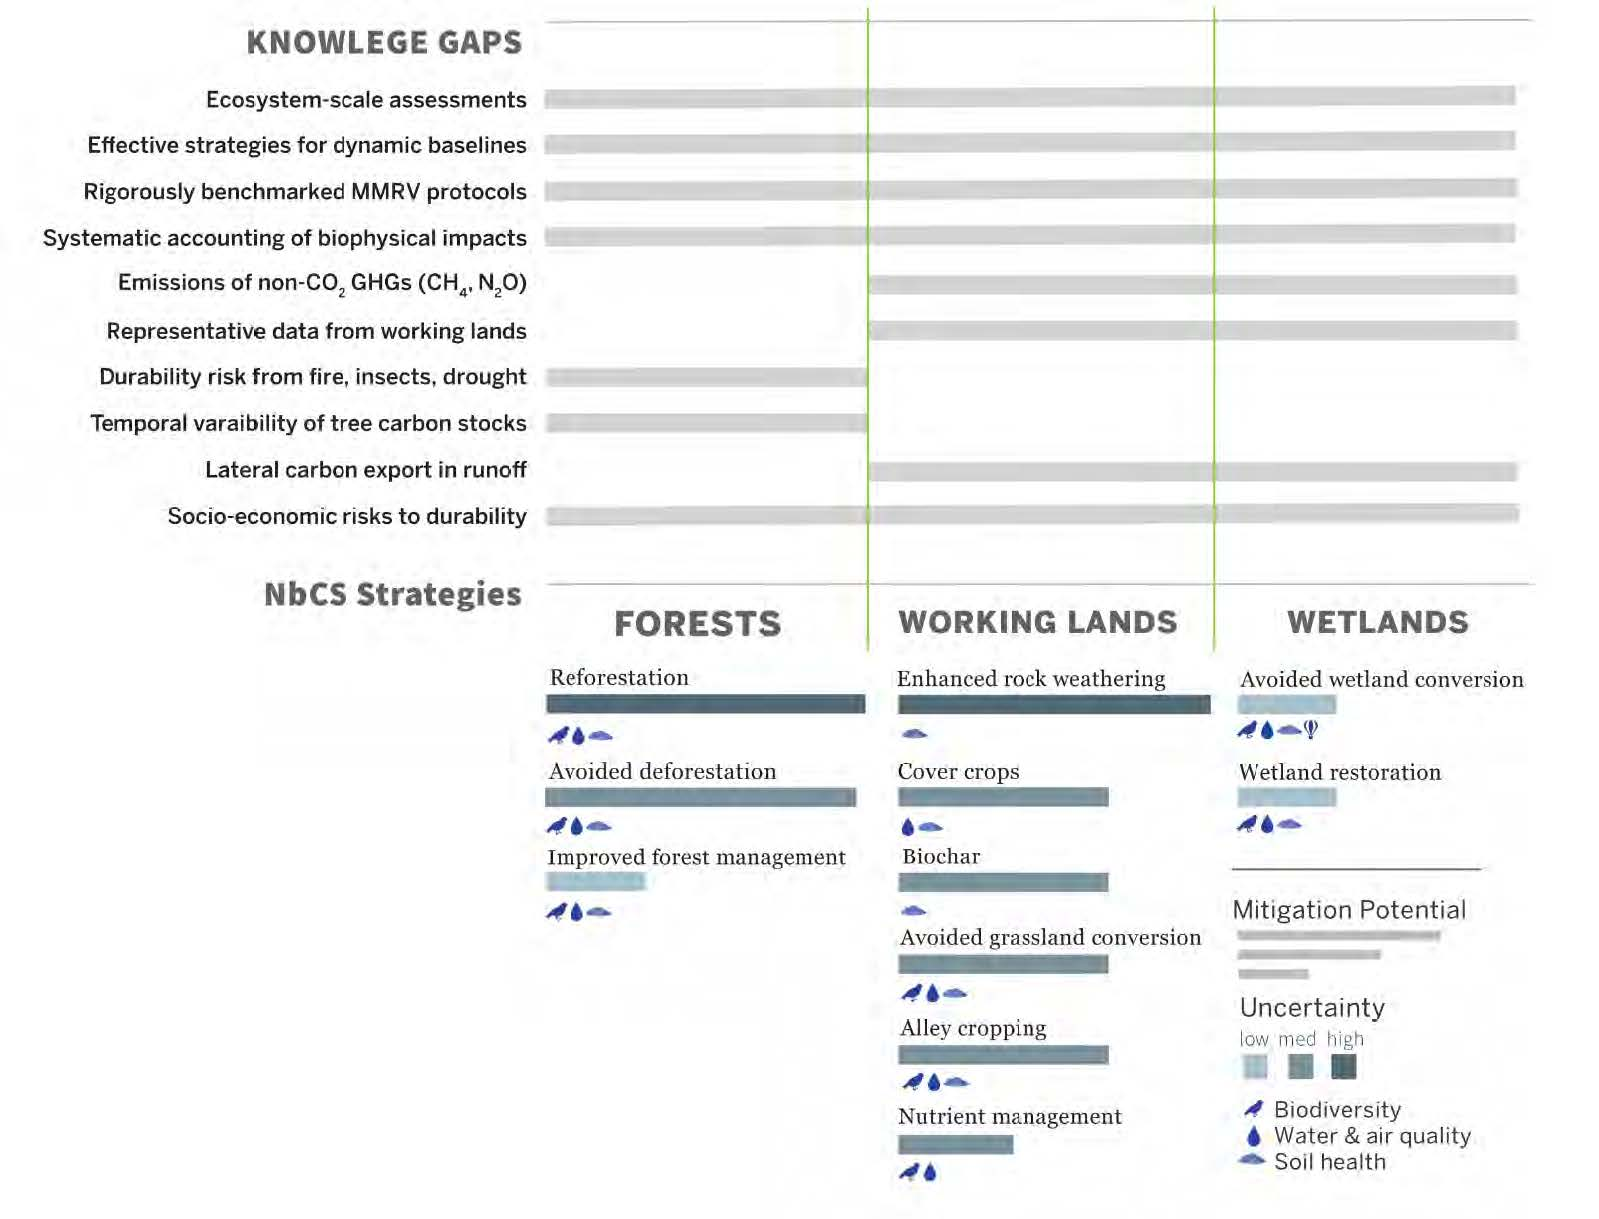
\includegraphics{img/01-nature-climate-solutions.jpg}

}

\caption{\label{fig-terrestrial-nature-solutions}In the bottom of the
figure, the length of the bar indicates (qualitatively) the expected
carbon mitigation potential, and the color represents uncertainty around
this potential. Icons indicating relevant co-benefits. Based largely on
information presented in Farigone et al.~201829. The top of the figure
highlights some of the most pressing knowledge gaps (see
Chapter~\ref{sec-overview} for more detail).}

\end{figure}

\hypertarget{sec-criteria}{%
\section{Key criteria, limitations, and
opportunities}\label{sec-criteria}}

While there is ample justification for implementing NbCS based on their
co-benefits alone, for NbCS to succeed specifically as climate
mitigation tools, they must meet four essential criteria:

\begin{itemize}
\tightlist
\item
  Criteria 1: Lead to enhancements to carbon uptake and/or reductions of
  non-CO2 GHGs that are additional to what would have occurred in a
  baseline or counterfactual scenario, and that integrate over all
  ecosystem sources and sinks.
\item
  Criteria 2: Lead to net cooling such that the biophysical effects on
  water and energy cycling do not overwhelm the gains in carbon uptake
  or emissions reductions.
\item
  Criteria 3: Achieve durable carbon storage by accounting for social
  and environmental risks to the permanence of ecosystem carbon storage
  and avoided GHG emissions.
\item
  Criteria 4: Account for leakage so that gains in one area are not
  canceled out by shifting activities to another area.
\end{itemize}

As discussed in detail in this report and elsewhere, major knowledge
gaps and concerns surrounding current NbCS activities and protocols
limit the extent to which they fulfill these criteria8,10,30,52,63,64
(Fig. 1). At regional and continental scales most relevant to
policy-setting, estimates of the present-day mitigation potentials of
NbCS vary substantially from one study to the next.2-4 These potentials
are usually estimated as a change in the amount of carbon residing in
two slowly evolving carbon stocks: shallow soil and aboveground plant
biomass. A focus on these two pools alone cannot capture the
ecosystem-scale carbon impacts of NbCS and tells us little about
emissions of non-CO2 GHGs (criteria 1). Moreover, for many NbCS,
existing data on how these stocks change are sparse and unrepresentative
of naturally occurring environmental gradients, limiting the available
information necessary to inform baselines against which additionality
can be calculated (criteria 1). A focus on changes in carbon stocks also
does not capture ``biophysical'' impacts of NbCS that can have both
favorable and unintended direct effects on temperature and water cycling
(criteria 2). Furthermore, the durability of carbon stored in soils and
woody biomass (criteria 3), as well as the leakage potential (criteria
4) are difficult to quantify and are not robustly considered in NbCS
accounting schemes. Together, these uncertainties reveal critical
challenges that hinder quantification of NbCS impacts from local to
continental scales, now and into the future.

Fortunately, substantial opportunity exists to address this uncertainty
by harnessing state-of-the-art carbon cycle measurement and prediction
tools together with lessons learned from practical experience in
implementing NbCS on the ground. The dominant role of terrestrial
ecosystems in determining atmospheric CO2 concentrations has been known
for decades. Consequently, huge investments of material resources have
fostered the development of innovative measurement technologies,
analytical tools, and predictive models for quantifying ecosystem carbon
cycles (Fig. 2). By and large, these tools have historically been used
for basic research of ecological processes and to inform global-scale
predictions for the future land carbon sink; but so far, the vast
majority have not been widely leveraged for what they might tell us
about expected and realized benefits of NbCS. Likewise, novel approaches
for crediting and verifying the climate benefits of NbCS are
proliferating at a range of scales, though most have not yet been widely
deployed61,62. Thus, right now, as we face a sea change in federal and
private-sector engagement with NbCS, we have a unique opportunity to
integrate the best-available science into next-generation information
systems to support effective NbCS programs and policy that address all
four key criteria.

\begin{tcolorbox}[enhanced jigsaw, title=\textcolor{quarto-callout-note-color}{\faInfo}\hspace{0.5em}{Box 1: Elements of robust, scalable, and credible NbCS}, colback=white, opacitybacktitle=0.6, arc=.35mm, breakable, rightrule=.15mm, titlerule=0mm, toptitle=1mm, colframe=quarto-callout-note-color-frame, left=2mm, bottomtitle=1mm, leftrule=.75mm, toprule=.15mm, coltitle=black, opacityback=0, bottomrule=.15mm, colbacktitle=quarto-callout-note-color!10!white]

\begin{itemize}
\tightlist
\item
  \textbf{Robust:} NbCS incentivization programs fully address all four
  key criteria (additional mitigation, net cooling, durability, and
  leakage). Doing so means that NbCS accounting schemes

  \begin{enumerate}
  \def\labelenumi{\arabic{enumi}.}
  \tightlist
  \item
    are informed by ecosystem-scale data that integrate over all carbon
    sources and sinks,
  \item
    consider a full set of GHG fluxes,
  \item
    explicitly account for the durability of carbon stored in soils and
    tree biomass and the possibility of leakage, and
  \item
    are holistic, considering not only the climate mitigation potential,
    but also coupled biophysical impacts on energy and water cycling.
  \end{enumerate}
\item
  \textbf{Scalable:} The strategies used to quantify the benefits of
  individual NbCS projects are harmonized with approaches to map the
  same benefits over regional and continental scales, so that NbCS
  programs can be informed by an understanding of when and where
  specific strategies are most likely to succeed.
\item
  \textbf{Credible:} The policy instruments used to incentivize NbCS
  rely on monitoring and quantification tools that are rigorously
  standardized and cross-compared, with open and transparent data and
  code sharing, allowing for independent validation of all activities
  and projections.
\end{itemize}

\end{tcolorbox}

\hypertarget{sec-path}{%
\section{A path forward}\label{sec-path}}

The objective of this report, which is co-authored by experts in both
NbCS science and implementation, is to describe the technologies, tools
and approaches necessary to support robust, scalable, and credible NbCS
strategies for the US. The report is organized around the identification
of key knowledge gaps and pathways to close them, providing a road map
for actionable, cross-sectoral information to foster NbCS strategies
that work while avoiding energy wasted on NbCS strategies that have
limited environmental benefits or the potential to backfire and
exacerbate climate change. The criteria for robust, scalable, and
credible NbCS defined in Box 1.

Before we proceed, there are two things to keep in mind. First, it is
important to distinguish between the concepts of ``technical mitigation
potential'' and ``realizable mitigation potential,'' which is sometimes
also referred to as ``social potential'' or ``economic potential.''
Technical mitigation potential describes increases in carbon uptake
and/or reductions in GHGs emissions that are theoretically achievable
through NbCS interventions, usually determined per unit area and summed
across all available areas. The factors that influence the technical
potential include heterogeneity in biophysical factors like climate,
species composition, and nutrient cycles, as well as uncertainties in
our ability to accurately measure changes in fluxes of CO2 and other
GHGs. The realizable mitigation potential includes other factors, such
as the sociological and economic forces that determine landowner
willingness to adopt or sustain a ``climate-smart'' practice. This
report is most strongly focused on research needed to quantify and
predict the technical mitigation potential of NbCS. Frequently, gaps and
research needs related to the realizable potential are also highlighted.

Second, the knowledge gaps that we identify in Section 2 are not trivial
and appear to reveal a wide gulf between the state-of-the-science
surrounding NbCS and the pace at which NbCS strategies are being
implemented on the ground. Indeed, there are many points of disconnect,
including a lack of consensus among scientists about the realizable
climate benefits of these strategies56, a dearth of representative data
necessary for more confident quantification of NbCS impacts, and the
fact that many protocols used for most NbCS project accounting were
developed decades ago and do not leverage the best-available science.
However, it is important to remember that terrestrial ecosystem ecology
is a well-established field of study, and over the decades, we have
gained a tremendous amount of knowledge about the mechanisms that drive
variability in ecosystem carbon, water, energy, and nutrient cycles.
Critically, we have also developed a wide variety of pre-existing
experimental sites, datasets, technologies, and analytical tools that
have not yet been fully leveraged for what they reveal about NbCS (see
Section 3). Thus, relatively subtle shifts in the research questions we
ask and the scale at which we ask them, combined with strategic
expansion of existing field sites and monitoring networks, could
substantially alleviate the burden of material resource investment
necessary to address these knowledge gaps (see details in Section 4).

\begin{figure}

{\centering 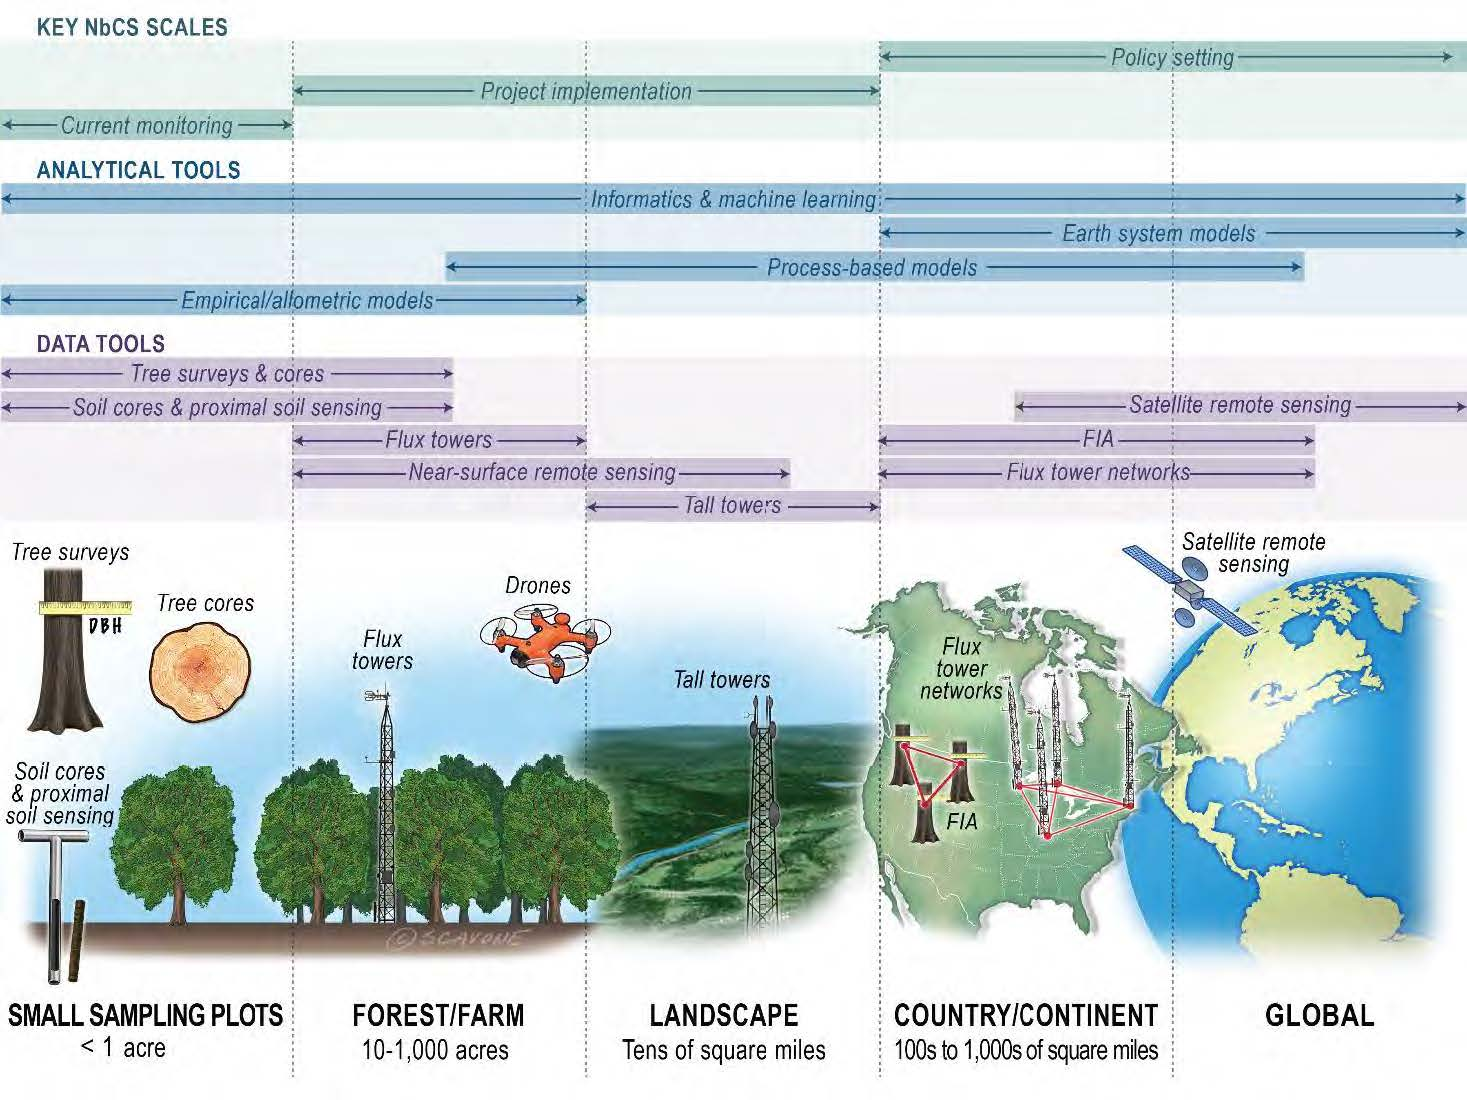
\includegraphics{img/02-nbcs-scales.jpg}

}

\caption{\label{fig-ncbsscales}The data and analytical tools that could
be more fully leveraged to inform NbCS. See Section 3 for details. Image
copyright William Scavone. All rights reserved.}

\end{figure}

\bookmarksetup{startatroot}

\hypertarget{sec-knowledge}{%
\chapter{Knowledge Gaps Limiting Robust, Scalable and Credible NbCS for
the United States}\label{sec-knowledge}}

\hypertarget{sec-data-scarcity}{%
\section{Knowledge gaps related to field data
scarcity}\label{sec-data-scarcity}}

Our understanding of the technical mitigation potential of many NbCS
strategies is limited by a scarcity of representative field data, either
because these data do not yet exist or because they are not yet freely
accessible. Notable exceptions exist, including networks of
ecosystem-scale flux towers (e.g., AmeriFlux65,66 and NSF's National
Ecological Observatory Network, or NEON67) and the wealth of information
on tree biomass and associated stand dynamics supported by the USDA
Forest Service Forest Inventory and Analysis (FIA) program68. These
networks may provide sufficiently representative data to map carbon
fluxes at coarse scales69, or even to estimate potential changes in
plant carbon stocks achievable with some NbCS like reforestation70,71.
However, networks like NEON, FIA and AmeriFlux were not designed
specifically with the goal of evaluating NbCS, and many specific NbCS
management strategies (e.g., cover crops, soil amendments, altered
forest management, wetland restoration) are potentially un- or
under-represented in these networks. These networks were also not
designed to be interoperable, which makes it difficult to blend
information from disparate networks (e.g., FIA and AmeriFlux) into
synthetic analyses and products. Efforts to dynamically catalog existing
NbCS field trials and the activities of relevant monitoring networks
would permit an informed prioritization of new data collection and
facilitate synthesis of new and existing network data.

Particularly in agricultural systems, there is a lack of scientific
consensus about the degree to which NbCS practices can sequester
sufficient atmospheric carbon to help mitigate climate change72-75. This
disagreement stems in part from a \textbf{large degree of uncertainty
surrounding the spatial and temporal patterns of soil organic carbon
(SOC) and net GHGs across agricultural landscapes76-80}. Field trials
for emerging NbCS strategies (e.g., enhanced rock weathering) are
scarce. However, there is even a lack of representative soil carbon
storage data for a practice like cover cropping, which has long been
known to confer multiple environmental benefits for soil health and
water quality81-83. One of the most widely cited papers reporting on the
soil carbon benefits of cover crops34 is informed by data from 37 sites
globally, with only 10 locations within the United States. Likewise,
although no-till management has long been lauded for its benefits to
soil health and for its role in reducing on-farm fossil fuel emissions,
the ability of no-till management to sequester atmospheric carbon has
been hotly debated in the scientific literature72,84. Some studies
conclude it has no potential to mitigate climate change, whereas other
research suggests that mitigation potential depends on climate and soil
texture85. Almost no data exists on the impact of multiple, or stacked,
NbCS farming practices despite the widespread use of stacking among
regenerative farmers. More data is needed from a much more
representative set of ecosystems to quantify where these practices
succeed as climate solutions, alone and in combination.

\textbf{The mechanisms by which agricultural practices impact coupled
carbon and nitrogen dynamics is another major knowledge gap.}
Understanding the net GHG impact of agricultural management demands data
on how specific practices impact both soil organic carbon (SOC) and
associated GHGs like nitrous oxide and methane. Agricultural practices
that build SOC can result in increased nitrous oxide emissions, which
could potentially offset gains in SOC sequestration86,87. Quantifying
potential trade-offs is difficult because nitrous oxide emissions vary
temporally and spatially and constitute a highly uncertain component of
agricultural GHG budgets87. In addition, practices which may reduce N2O
from fertilizer or manure application may adversely affect other parts
of the nitrogen cycle and increase ammonia loss88. \textbf{We need
increased data coverage over time and space to more accurately quantify
the net GHG impacts and additional positive or negative effects of
agricultural management practices.} These databases could build onto and
complement USDA Agricultural Research Service GHG synthesis projects
such as TRAGNET89 and GRACEnet90,91.

Our understanding of NbCS potentials in agricultural landscapes moreover
requires data from working farms. Much of our knowledge about management
impacts on SOC sequestration comes from long-term agricultural field
trials designed to minimize inherent variability in soils and landscape
position that exists in the real-world92. Thus, estimates of SOC
sequestration rates are often greater than those measured at the farm
scale93, and practices as implemented in 2. Knowledge Gaps Limiting
Robust, Scalable and Credible NbCS for the United States 10 research
trials (e.g., long-term no-tillage) might not reflect how these
practices are implemented in practice by farmers (e.g., intermittent
tillage). A network of sites (ideally containing paired fields
evaluating different practices) that collect data on management records,
soil properties, climate data, crop yields, carbon fluxes, and nitrogen
fluxes could help build external validity of agricultural management
impacts on net GHG outcomes.

Many of these field data limitations also apply to terrestrial wetland
ecosystems, which have additional, unique knowledge gaps. There is still
a need to better map wetlands94 and to locate restoration and conversion
avoidance opportunities more precisely. Next, emissions and carbon
trajectories associated with different wetland conditions and
restoration strategies need to be rigorously quantified. The use of eddy
covariance combined with long-term, plot-level measurements of GHG
emissions are important tools to fill this gap95, though wetlands are
relatively underrepresented in networks like AmeriFlux and NEON96.
Wetlands also pose measurement difficulties as they are a mosaic of
water and vegetation with stark gradients in nutrients, plant species,
soil saturation and salinity (for estuaries) that can impact carbon
cycling and GHG emissions97-99. Getting the fluxes right at the
field-scale requires a mix of measurement and gap-filling approaches and
high-resolution remote sensing100,101. It is also important to consider
socioeconomic factors, including the design of locally appropriate
incentive programs that account for competing land uses and the multiple
ecosystem services102,103, plus impacts associated with disturbance104.

Especially in wetland environments and the tile-drained croplands that
predominate the Corn Belt, more information is required regarding
potentially significant leakage through lateral transport of dissolved
and particulate carbon105-107. A change in SOC may represent an increase
in carbon sequestration from the atmosphere, but it may also represent a
decrease in carbon losses through runoff and leaching. Depending on the
fate of carbon exported in this way, an increase in soil carbon may not
represent atmospheric CO2 sequestration of the same magnitude.
Unfortunately, information about lateral export of carbon, especially in
places where carbon pools and fluxes are already being measured, is
scarce and largely unaggregated into network databases.

Field data on the carbon contained in forests are relatively more
plentiful, due in large part to the FIA program. Indeed, FIA data have
played a central role in governing our understanding of the dynamics of
carbon stored in tree biomass, and FIA biomass data are featured in most
attempts to quantify the mitigation potential of reforestation in the
U.S.31,70,108-110. However, FIA was not designed explicitly for the
purpose of documenting how a limited set of management strategies will
alter the GHG flux balance of America's forests. For example, while SOC
has been measured on a subset of FIA plots111, \textbf{data on
\textbf{\emph{changes in soil carbon}} are not yet available from FIA.}
Moreover, the FIA network is characterized by long resampling intervals
(5-10 years) and protocols that lack rigorous documentation of the
causes of tree mortality or regeneration of young trees. These
limitations make it difficult to disentangle the influence of multiple
drivers of forest carbon dynamics that act simultaneously, including
climate variability and change, natural disturbances, forest harvest,
the CO2 fertilization effect, and their interactions. Furthermore,
\textbf{whether distributed plot networks like FIA adequately capture
the carbon cycle impacts of patchy disturbances, particularly fire and
beetle outbreaks, is also a major unknown.}

\begin{tcolorbox}[enhanced jigsaw, title=\textcolor{quarto-callout-important-color}{\faExclamation}\hspace{0.5em}{Box 2.1: Knowledge gaps related to data scarcity}, colback=white, opacitybacktitle=0.6, arc=.35mm, breakable, rightrule=.15mm, titlerule=0mm, toptitle=1mm, colframe=quarto-callout-important-color-frame, left=2mm, bottomtitle=1mm, leftrule=.75mm, toprule=.15mm, coltitle=black, opacityback=0, bottomrule=.15mm, colbacktitle=quarto-callout-important-color!10!white]

\textbf{Gap 2.1a:} Many categories of NbCS are under-represented in
existing networks, and field trial data are scarce.

\textbf{Gap 2.1b:} The absence of long-term monitoring data on soil
carbon in agricultural working lands limits consensus on when and where
many NbCS are most likely to succeed.

\textbf{Gap 2.1c:} Unrepresentative data on coupled soil carbon and
nitrogen dynamics, and lateral carbon transport, limits evaluation of
inherent tradeoffs (e.g.~carbon versus methane and nitrous oxide,
sequestration versus runoff).

\textbf{Gap 2.1d:} The design of existing forest inventory programs
limits understanding of carbon stored in soils, litter, and dead wood,
and precludes attribution of tree growth and mortality to disturbances
and management. In addition, some disturbance such as wildfire may be
incompletely captured with a distributed plot sampling network.

\end{tcolorbox}

\hypertarget{sec-carbon}{%
\section{Knowledge gaps related to a historic emphasis on a limited set
of carbon stocks}\label{sec-carbon}}

Even if data are plentiful, substantial additional uncertainty can be
traced to a historic emphasis on two slowly evolving carbon stocks (or
pools); specifically, {[}1{]} soil carbon in the top 30 cm of the soil
in croplands and grasslands, and {[}2{]} and the carbon contained in
aboveground plant biomass. Approaches for estimating the carbon
contained in a soil sample, or in a single tree, are well established.
In the case of soil carbon, small soil cores are physically extracted
from the soil and analyzed for their carbon content in the laboratory.
For tree carbon, field measurements of tree diameter and height are
collected and used as inputs into empirical (allometric) relationships
that describe species-specific relationships between tree size and
carbon content. While the accessibility of these measurements is
advantageous, linking the mitigation potential of NbCS solely to
present-day changes in these pools remains limited in three major ways.

First, a narrow focus on only two pools misses important carbon sources
and sinks and prevents ecosystem-scale assessments of NbCS
impacts7,112,113 (Fig. 3). Soils store a large proportion of carbon in
the sub-surface (depths \textgreater{} 30 cm). Yet research on soils has
focused on the surface (0-30 cm) as the zone of greatest biological
activity that responds most readily to management, and nearly all
crediting systems only model or measure down to 30 cm or less55,114.
Studies that have captured greater depths reveal that certain practices
like no-till farming result in a redistribution of SOC such that
perceived gains in surface soils may be attenuated by losses at
depth84,115,116. The lack of data on SOC dynamics at depth hinders our
ability to draw robust conclusions and uncertainty remains high117-119.

In the case of tree carbon, allometric relationships linking tree size
and carbon content are typically based on trees that were harvested
decades ago. Thus, these allometric models may not incorporate the many
ways that climate feedbacks like rising atmospheric CO2 and increasing
drought stress can affect patterns of tree growth and allocation120-121.
Moreover, while tree biomass is often the fastest-growing pool of carbon
in forests, forest soil carbon is a dynamic pool in which most forest
carbon resides123. A non-negligible quantity of carbon assimilated by
trees is ultimately translocated to and stored in the soil each year
through root exudates, leaf litter, and inputs from downed woody
debris122. Moreover, in a world characterized by more frequent tree
die-offs, the rates of accumulation in standing and downed dead biomass
carbon stocks could increase. Indeed, over the past 10 years, the downed
wood biomass of forests in the contiguous U.S. has increased 18\% while
live biomass has increased only 4\%123. Finally, a growing body of
literature suggests that the link between stem biomass increment and
tree carbon uptake (e.g., net primary productivity) is not particularly
strong124126. Taken together, these considerations motivate forest NbCS
assessment and accounting protocols that consider ecosystem-scale fluxes
and a larger set of carbon pools.

Second, because ecosystem carbon pools are quite large to begin with, it
can take years for a change in these pools to become detectable, whereas
a change in the land-atmosphere flux can be detected immediately. To
understand this limitation, it can be helpful to visualize a swimming
pool, representing all the carbon in an ecosystem. Imagine the pool is
being filled by a hose (representing the net flux of CO2 from the
atmosphere to the ecosystem), and that there is negligible outflow from
the pool (e.g., leaks like the lateral loss of carbon through runoff are
small). If the hose inflow rate is doubled (representing the
implementation of an NbCS strategy), an observer tracking inflow from
hose will be able to quantify the impact of the intervention
immediately. However, an observer attempting to infer this flux by
tracking changes in the volume of water in the pool will have to wait
much longer for the change in inflow to become detectable. Most NbCS
accounting and crediting protocols are focusing on the pool, and not the
hose. This mismatch has important consequences for the speed with which
the climate benefits of individual projects can be quantified. A
multiyear delay in understanding if an NbCS treatment is producing the
desired outcomes increases uncertainty in implementation programs and
limits our ability to rapidly evaluate the effectiveness of emerging
NbCS strategies.

Together, these first two issues point to advantages and disadvantages
of both flux and stock measurement and detection techniques (Fig. 3). In
isolation, ecosystem-atmosphere flux observations are unable to track
where carbon is stored in an ecosystem (an important determinant of
durability) or the potential for rapid off-site release of recently
sequestered CO2 (e.g., following harvest or lateral export in runoff).
Stock change measurements can be ambiguous regarding where carbon comes
from and goes to, and may not differentiate between increases in inputs
or decreases in outputs. For example, an increase in soil carbon might
result from increased litter production because of stimulated plant
growth, which would cause a reduction in atmospheric CO2, or from
enhanced litter production due to disturbance, which would not lower CO
2 concentrations. Both stock and flux approaches are incomplete without
the other. We need confident tracking of carbon fluxes and stock changes
with holistic tracing of carbon flows throughout the system.

\begin{figure}

{\centering 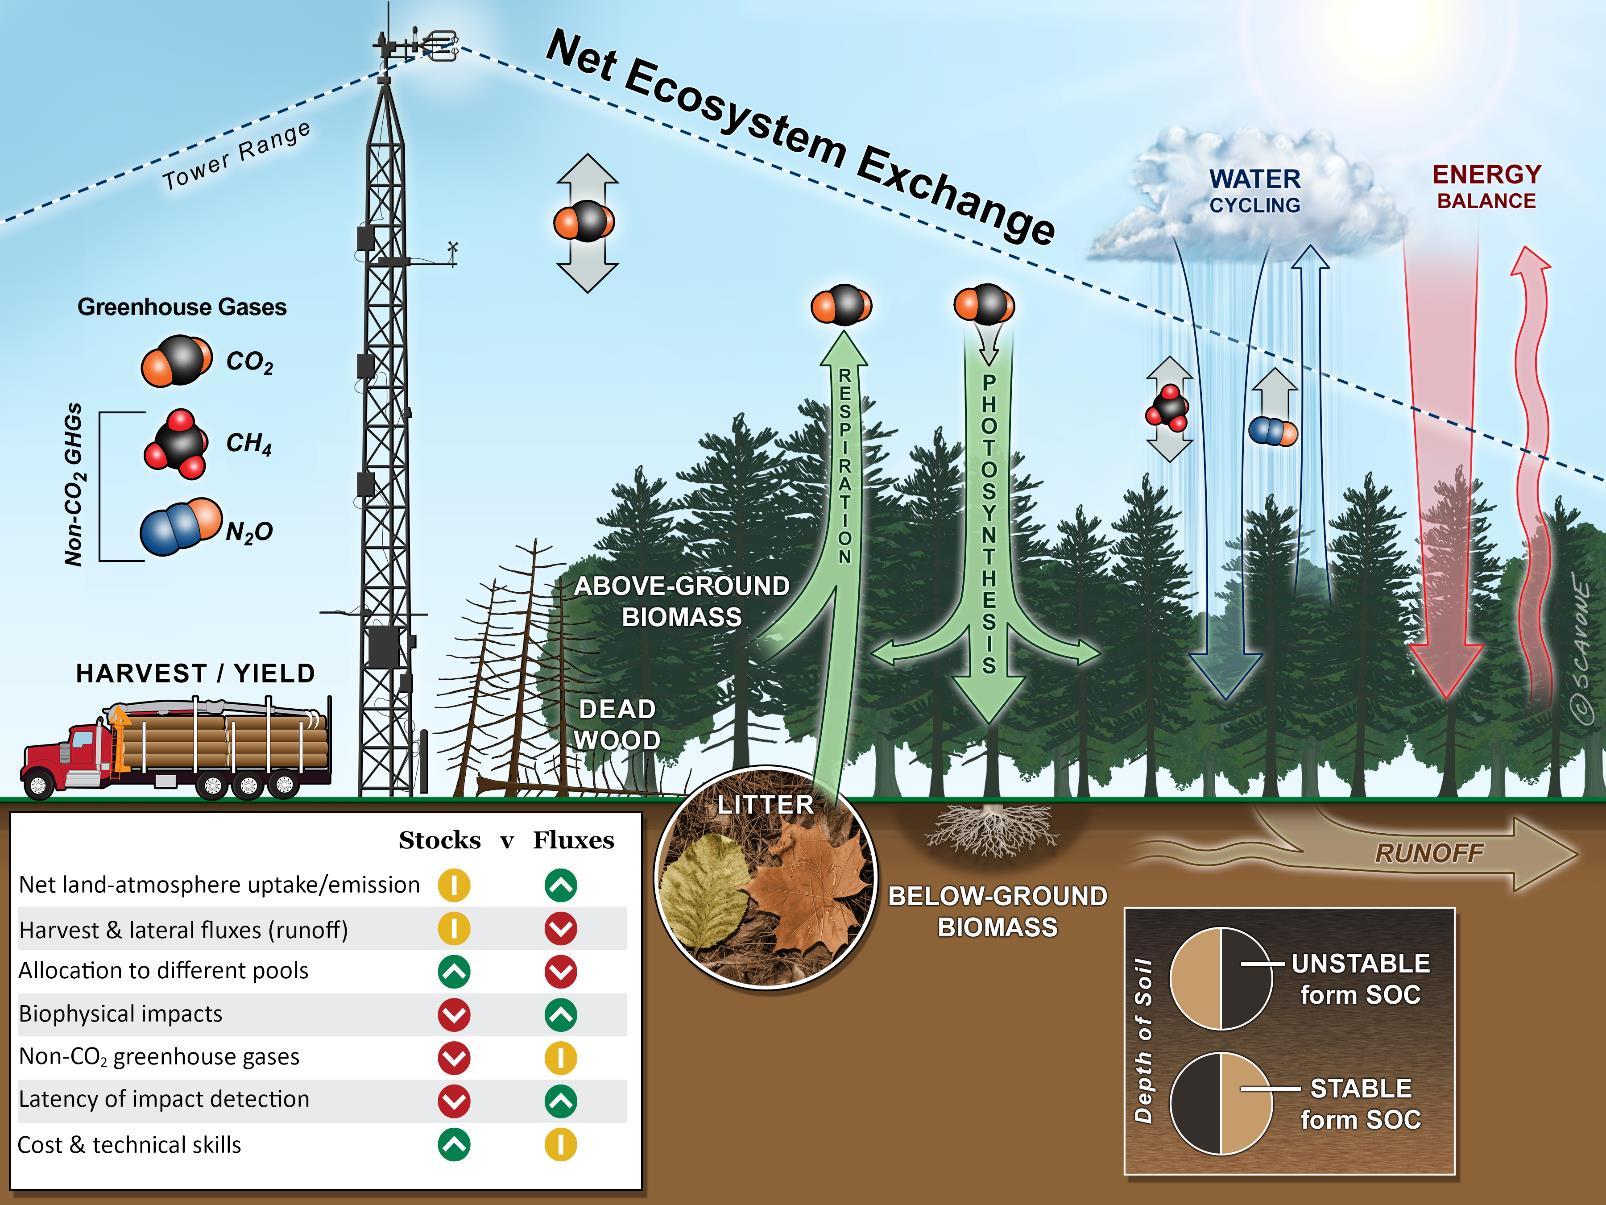
\includegraphics{img/03-ecosystem-fluxes-stocks.jpg}

}

\caption{\label{fig-key-fluxes-stocks}Flux towers provide
ecosystem-scale measurements of the net ecosystem exchange of CO2
between the land and the atmosphere, and some towers can also measure
the land-atmosphere flux of methane and nitrous oxide. Because towers
record information continuously, they can landsome atmosphere flux of
methane and nitrous oxide. Because towers record information
continuously, they can quickly detect the impact of changes in land
cover and management, especially when deployed in an experimental
setting. Their ability to continuously measure ecosystem-scale water and
energy fluxes also makes them particularly useful for understanding
biosphysical impacts. However, flux towers are not able to monitor
carbon lost to harvest or runoff, and provide little information about
the allocation of sequestered carbon to different pools. On the other
hand, changes in ecosystem stocks will reflect the combined influence of
inputs (e.g., sequestration/emission) and outputs (e.g., harvest/runoff)
on pool sizes. Depending on how many pools are monitored, theses
observations also provide more granular information about how
sequestered carbon is allocated (e.g., to above versus belowground
pools, including more stable versus more unstable forms of SOC). For
these reasons, flux and stock measurements are best viewed as
complimentary. The table in the lower left illustrates the relative
advantages and disadvantages of each approach. Green symbols indicate an
advantage, red symbols indicate a disadvantage, and yellow symbols
indicate that the relative design. Image copyright William Scavone. All
rights reserved.}

\end{figure}

Third, focusing on carbon stocks alone prevents a more holistic
understanding of the overall GHG emission benefits (or unintended
consequences) of a given NbCS strategy. Specifically, carbon stock
changes are insufficient to understand NbCS impacts on emissions of
non-CO2 GHGs like methane and nitrous oxide, which are particularly
important to consider in wetlands and many agricultural systems. We
urgently need strategies to resolve NbCS-driven changes to these GHGs
with a precision that overcomes uncertainty due to natural variability.

\begin{tcolorbox}[enhanced jigsaw, title=\textcolor{quarto-callout-important-color}{\faExclamation}\hspace{0.5em}{Box 2.2: Knowledge gaps related to a historic emphasis on a limited set
of carbon stocks}, colback=white, opacitybacktitle=0.6, arc=.35mm, breakable, rightrule=.15mm, titlerule=0mm, toptitle=1mm, colframe=quarto-callout-important-color-frame, left=2mm, bottomtitle=1mm, leftrule=.75mm, toprule=.15mm, coltitle=black, opacityback=0, bottomrule=.15mm, colbacktitle=quarto-callout-important-color!10!white]

\textbf{Gap 2.2a:} NbCS assessments and protocols lack ecosystem-scale
perspectives that integrate over all relevant carbon sources and sinks.

\textbf{Gap 2.2b:} Limited ability to quickly quantify the actual
benefit of NbCS on the ground.

\textbf{Gap 2.2c:} Limited undrestanding of NbCS impacts on methane and
nitrous oxide emissions.

\end{tcolorbox}

\hypertarget{sec-mapping}{%
\section{Knowledge gaps preventing policy-relevant mapping of NbCS
mitigation potentials}\label{sec-mapping}}

The potential climate benefits of a given NbCS strategy will vary from
one location to the next, reflecting differences in climate, underlying
soils, topography, and historic management regime. If the goal is to
incentivize NbCS to maximize their climate benefits, the most robust
NbCS implementation programs would be designed with an understanding of
where and when a given strategy is most likely to succeed and would
avoid allocating resources to interventions that do not offer tangible
climate benefits. Unfortunately, spatially explicit maps of climate
change mitigation benefits for most NbCS strategies are scarce. This is
especially true for agricultural and wetland NbCS. At the time of this
writing, to our knowledge, there are no published maps that rigorously
describe the carbon uptake benefits, or biophysical impacts, of cover
crops across the Corn Belt. Overall, a major factor limiting our ability
to map the climate benefits of agricultural and wetland NbCS is a lack
of representative data that spans many axes of variability (e.g., soils,
climate, species, historic management, land ownership history).

There are a couple of exceptions. No-till agriculture has been widely
studied through paired plot experiments, motivating several
meta-analyses that incorporate field data into models that relate
changes in soil carbon to mappable environmental drivers, yielding
spatially explicit estimates of carbon sequestration potential127,128.
However, recent work reveals that the change in soil carbon under
no-till management varies as a function of both time and depth into the
soil; and efforts to extrapolate estimates of the change in soil carbon
to regional- and continental-scale may lead to misleading
conclusions116. Likewise, mitigation potential maps of forest-based
strategies -- and especially reforestation -- are relatively abundant.
Data on aboveground biomass provided by inventory networks like FIA are
fairly complementary with remotely-sensed proxies for forest biomass
(e.g.~from GEDI129) as well as a suite of existing models and carbon
monitoring frameworks130,131 that predict carbon uptake based largely on
changes in biomass. Nonetheless, mitigation potential maps will only be
as robust as the underlying data; if these maps are informed primarily
by changes in carbon stored in shallow soils and/or aboveground woody
biomass, they will suffer from the same limitations described in the
preceding section.

The spatial resolution of mitigation potential maps will ultimately be
determined by the representativeness of the ground data used to train
the scaling algorithms, and the resolution of the remote sensing
products and models used for extrapolation. Maps at a resolution that
matches the scale of individual farms and forest stands are likely
infeasible in the near term. However, maps made at relatively fine
scales (e.g.~county-scale) may be possible for some NbCS strategies.

\begin{tcolorbox}[enhanced jigsaw, title=\textcolor{quarto-callout-important-color}{\faExclamation}\hspace{0.5em}{Box 2.3: Knowledge gaps preventing policy-relevant mapping of NbCS
mitigation potentials}, colback=white, opacitybacktitle=0.6, arc=.35mm, breakable, rightrule=.15mm, titlerule=0mm, toptitle=1mm, colframe=quarto-callout-important-color-frame, left=2mm, bottomtitle=1mm, leftrule=.75mm, toprule=.15mm, coltitle=black, opacityback=0, bottomrule=.15mm, colbacktitle=quarto-callout-important-color!10!white]

\textbf{Gap 2.3a:} Especially in agricultural and wetland systems, we
lack spatially-resolved maps of NbCS mitigation potentials, preventing
an understanding of when and where these strategies are most likely to
succeed. This gap is linked to a scarcity of representative ecological
and socio-economic data.

\textbf{Gap 2.3b:} In forests, existing potential maps are primarily
informed by data on tree biomass change, which miss other important
carbon pools.

\end{tcolorbox}

\hypertarget{sec-holistic}{%
\section{Knowledge gaps preventing a holistic assessment of NbCS
biophysical impacts}\label{sec-holistic}}

Any intervention designed to affect carbon cycling will have a
concomitant impact on water and energy cycling (hereafter ``biophysical
impacts''), as these three cycles are closely coupled132. For example,
due to the link between photosynthetic capacity and stomatal
conductance133, greater ecosystem photosynthesis is typically associated
with greater evapotranspiration46. All else being equal, an increase in
evapotranspiration is likely to decrease soil moisture and runoff.
Whether this is a favorable outcome greatly depends on the local climate
regime, time of year, and management goals. For example, greater
springtime evapotranspiration (e.g., linked to cover crop use) may be
welcomed by producers throughout much of the Corn Belt, where saturated
conditions can delay or even prevent planting of cash crop seeds134.
Conversely, when and where soil moisture deficits are common and limit
agro-ecosystem productivity, alterations to the hydrologic cycle that
further deplete soil moisture would be undesirable. With some
exceptions46,135,136, systematic frameworks for understanding how NbCS
impact carbon and water cycles are rare, and more holistic assessments
of coupled carbon-water impacts of NbCS are urgently needed. This is
also critical for ensuring water management strategies are consistent
and complementary with climate mitigation efforts, especially as water
availability becomes less predictable.

Land cover and management shifts also affect energy budgets in ways that
can impact temperature directly137. For example, replacing relatively
light colored (high albedo) grasslands with darker (low albedo) forests
will increase solar radiation absorbed at the surface, which can have a
local warming effect. However, at the same time, forests tend to use
more water (higher evapotranspiration) and generate more effective
transport of heat energy away from the land surface (increased sensible
heat flux). Both mechanisms tend to cause surface cooling at local
scales138,139.

Arguably, for some categories of NbCS, our understanding of local
temperature impacts is more advanced than our understanding of carbon
cycle impacts. While no remote sensing platform is yet capable of
sensing the net carbon flux directly, satellite estimates of land
surface temperature and surface albedo have been widely available for
decades. Moreover, flux towers measure all the relevant terms of the
ecosystem energy budget. When deployed in a paired-site setting139,140,
flux towers can tell us not only how local surface temperature is
affected by a land cover or management shift, but also which underlying
mechanisms are responsible for the shift138,139,141,142 Collectively,
these data products have been widely used to demonstrate that NbCS
strategies in some regions have an overall local surface cooling effect
(e.g., tropical and temperate zone reforestation135,143,144; wetland
restoration145, and conversion to frequently flooded agriculture
lands146). In other cases (e.g., semi-arid and boreal forests), the
radiative impacts of NbCS may lead to additional warming141,147.
Nonetheless, the consequences for local surface temperature have not
been rigorously quantified for many categories of NbCS. For all NbCS
strategies, more work is necessary to understand the relationship
between local surface and air temperature impacts148,149, especially
during climate extremes like heat waves150,151.

Importantly, local temperature responses to NbCS do not necessarily
scale up to regional or global temperature changes. In isolation, a
decrease in albedo will tend to cause both local and global warming. To
the extent that NbCS increase evapotranspiration that results in
increased cloudiness, they may cause reductions in planetary albedo
which has a cooling effect137. But on the other hand, heat diverted from
the surface through enhancements to evapotranspiration and sensible heat
flux is re-released in the atmosphere and does not escape the planetary
climate system. Consequently, changes in local surface temperature are
not necessarily correlated with a global climate system response, making
changes in local surface temperature an incomplete indicator of the
biophysical impacts of NbCS131,152,153. Although these mechanisms are
broadly understood by meteorologists and climate scientists, they are
not always considered by practitioners or even some scientists working
with NbCS.

Finally, evidence from modeling studies suggests that modifications to
energy and water cycling in one location can have downstream effects on
water and energy cycling in other locations through non-local effects
and so-called ``eco-climatic teleconnections''154,155. Right now, our
understanding of these non-local effects is limited to what we can learn
from climate models, which often struggle to characterize resulting
temperature changes with sufficient precision to match the scale of NbCS
interventions.

\begin{tcolorbox}[enhanced jigsaw, title=\textcolor{quarto-callout-important-color}{\faExclamation}\hspace{0.5em}{Box 2.4: Knowledge gaps related to biophysical impacts}, colback=white, opacitybacktitle=0.6, arc=.35mm, breakable, rightrule=.15mm, titlerule=0mm, toptitle=1mm, colframe=quarto-callout-important-color-frame, left=2mm, bottomtitle=1mm, leftrule=.75mm, toprule=.15mm, coltitle=black, opacityback=0, bottomrule=.15mm, colbacktitle=quarto-callout-important-color!10!white]

\textbf{Gap 2.4a:} We lack a comprehensive framework for understanding
how NbCS impact local water cycling.

\textbf{Gap 2.4b:} For most categories of NbCS, we lack a rigorous
quantification of biophysical impacts for surface and air temperature at
local to planetary scales.

\textbf{Gap 2.4c:} Climate and land surface models struggle to reproduce
the direct temperature impacts of NbCS with enough precision to quantify
local and non-local biophysical impacts.

\end{tcolorbox}

\hypertarget{sec-durable}{%
\section{Knowledge gaps limiting predictions of durability and
disturbance risk}\label{sec-durable}}

\hypertarget{sec-robust-ncbs}{%
\subsection{The importance of durability for robust
NbCS}\label{sec-robust-ncbs}}

Durability refers to the period of time over which carbon removals or
avoided emissions that result from an NbCS intervention persist without
failure. The term is used in practice to characterize the duration for
which carbon mitigation from a particular policy, market, or program is
assured to remain out of the atmosphere. Durability depends on relevant
physical and ecological risk factors that can lead to ``reversals''
through which carbon or other GHGs return to the atmosphere. For
example, carbon stored in forests is vulnerable to mortality events
driven by wildfire, drought, disease, and insects156. In many instances,
durability also depends significantly on program governance features50,
such as whether a parcel of land has committed to maintain climate-smart
practices by contract or by easement, as well as whether a program
includes insurance mechanisms to address reversal risks157. As a result,
properly characterizing the durability of NbCS requires insights from
natural and social sciences, as well as assessments of environmental
economics and policy.

\bookmarksetup{startatroot}

\hypertarget{references}{%
\chapter*{References}\label{references}}
\addcontentsline{toc}{chapter}{References}

\markboth{References}{References}

\hypertarget{refs}{}
\begin{CSLReferences}{1}{0}
\leavevmode\vadjust pre{\hypertarget{ref-novick-et-al22}{}}%
Novick, Kim, Christopher Williams, Benjamin Runkle, William Anderegg,
Dave Hollinger, and Marcy Litvak. 2022. {``The Science Needed for
Robust, Scalable, and Credible Nature-Based Climate Solutions for the
United States: Full Report.''} Bloomington: Indiana University Libraries
Department of Scholarly Communication.
\url{https://doi.org/10.5967/n7r9-7j83}.

\leavevmode\vadjust pre{\hypertarget{ref-walker-et-al19}{}}%
Walker, Xanthe J., Jennifer L. Baltzer, Steven G. Cumming, Nicola J.
Day, and Christopher Ebert. 2019. {``Increasing Wildfires Threaten
Historic Carbon Sink of Boreal Forest Soils.''} \emph{Nature}, no. 572.

\end{CSLReferences}



\end{document}
